% \section{Fixed step solver}
% \subsection{Test Equation}
% \begin{figure}[h!]
% 	\centering
% 	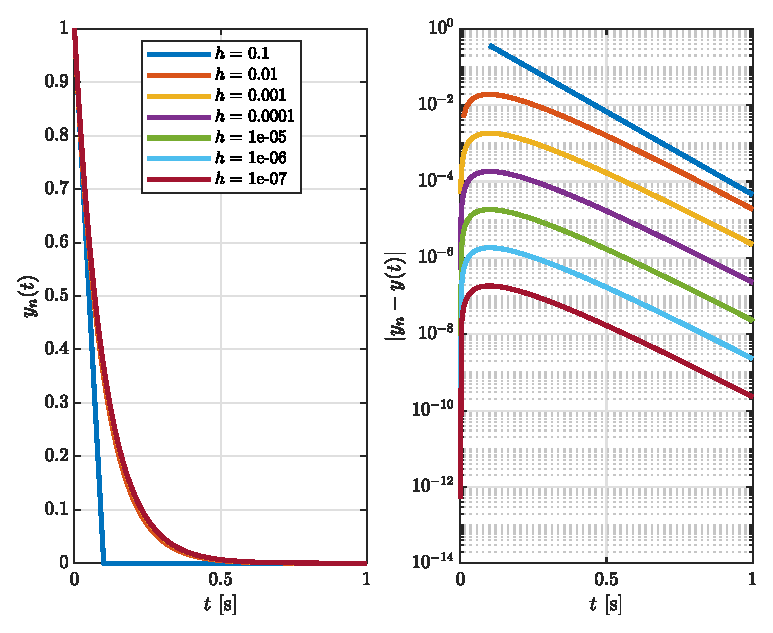
\includegraphics[width=\textwidth]{Figures/ef_testCase.eps}
% 	\caption{Simulation of the test equation using the Euler forward method with $\lambda=1$.}
% 	\label{fig:testEF}
% \end{figure}
% The consistency of the Euler forward method is checked by using a test equation. The test equation is given as follows:
% \begin{align*}
% 	\textbf{Test equation: }f(t,y) &= -\lambda\,y, \quad y(0) = 1. & \textbf{Analytical solution: } & y = e^{-\lambda\,t}.
% \end{align*}

% Using the test equation, the solver's (or numerical method's) \textit{convergence} is checked.

% \subsubsection{Convergence}
% The solver arrives at a solution that is close to the exact solution within some pre-specified error tolerance or other convergence criterion. This is the significance of convergence. % This is the, indeed,goal of the project. 

% By definition, the solver is said to be \textit{convergent of order $p$} if the global error $e_n$, satisfies
% \begin{align*}
% 	e_n = O(h^p)
% \end{align*}

% The simulation results of the test equation are presented in \prettyref{fig:testEF}. From the figure, the order of the system is calculated and presented in the table below:
% \begin{table}[h!]
% 	\centering
% 	\begin{tabular}{c|c|c}
% 		h & $|y_n - y(t)|$ & $p$ \\
% 		\hline
% 		0.1 & 1.58e-3 & \\
% 		0.01 & 1.67e-4 & 0.95\\
% 		0.001 & 1.68e-5 & 0.99 \\
% 		0.0001 & 1.68e-6 & 1 \\
% 		1e-5 & 1.69e-7 & 1 \\
% 		1e-6 & 1.69e-8 & 1 \\		
% 		1e-7 & 1.69e-9 & 1 	
% 	\end{tabular}
% \end{table}\\
% From the table and the figure, it is clear that, as $h\rightarrow0,\ |y_n - y(t)| \rightarrow0$. Therefore, according to the fundamental convergence theorem, the solver is \textit{convergent of order $p$}. % Furthermore, is can also be observed that the solver is also \textit{consistent} and also \textit{0-stable}. 

\subsection{Simulation with fixed-step solver}
\begin{figure}[t!b!]
	\centering
	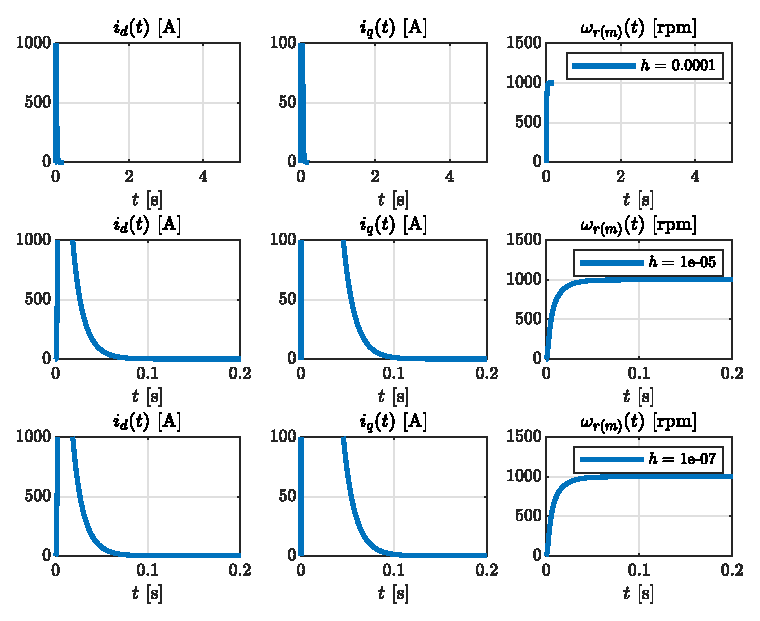
\includegraphics[width=\textwidth]{Figures/ef_MotorCase.eps}
	\caption{Simulation of the PMSM using Euler forward method with $\vd=\vq=800\,$V at three different step sizes, $h = 0.001$, $h = 1\text{e}-5$, and $h = 1\text{e}-7$ .}
	\label{fig:EMresEF}
\end{figure}
\prettyref{fig:EMresEF} presents the simulation results of a PMSM using the \textit{forward Euler} method. The figure shows the states (dynamic variables) \id, \iq, and \wm as a function of time. From the figure, it is clear that as $h \rightarrow 0$. all the states converge to a constant value. The time constant of the current transient (\Ld/\Rs) is about $9.9\text{e}-4$\,s. The minimum step size should be below this for the solver to converge. 

\fbox{\parbox{0.98\textwidth}{
\emph{When should one use $h = 1\text{e}-5$, and $h = 1\text{e}-7$?} \\
if the goal is to analyze the steady state of the speed, i.e., after 0.5\,s, then $h = 1\text{e}-5$ is sufficient. If the goal is to get very accurate information about the current transient, lower $h$ is better.

\emph{Why can we trust the results?} \\
As $h \rightarrow 0$, the current transient peak and the time constant reaches closer to (\Ld/\Rs) is about $9.9\text{e}-4$\,s. Furthermore, the errors both during the transients and steady states reduce as $h \rightarrow 0$. Therefore, we can trust the results, because they align with the theory of \textit{convergence}, as $h \rightarrow 0$, the numerical solutions are close to the true solution. 
}}

% This implies that % that the solver is \textit{0-stable}. Furthermore, it is also clear that 
% the ODE system is stable. 

% The \textit{convergence} of the numerical method was checked in the previous section. Therefore, it can be concluded that the simulated results with $h \leq 1\text{e}-4$ gives the a solution that is very close to the true solution to the ode system.

%\subsubsection{Validation from control theory}
%During steady state operation on the PMSM, i.e, 1\,s simulation time, the \texttt{odes} (8), (9), and (10) can be simplified, as follows:
%\begin{align}
%	\Rs\,\id - \vd &= \Lq\,\iq\,\wm, & \vq - \Rs\,\iq &= \left(\Ld\,\id + \flux\right)\,\wm, & \Tl\,\frac{2\,K^2}{3\,\np} &= \iq\,\left(\left(\Ld - \Lq\right)\,\id + \flux\right), \label{eq:simlified}
%\end{align}
%Substituting the initial conditions for the simulation in \prettyref{eq:simlified}, we get:
%\begin{align*}
%	\iq &= 0
%\end{align*}

%The error at $t_N$ is given in the table below:
%\begin{table}[h!]
%	\centering
%	\begin{tabular}{c|c|c|c}
%		h & $|\id_N + j\,\iq_N|$ & \Te\textsubscript{\textit{N}} & \Nr\textsubscript{\textit{N}}\\
%		\hline
%		0.001 & $\infty$ & $\infty$ & $\infty$ \\
%		0.0001 & $3.18$e$-10$ & $5.3$e$-9$ & $1000.01$ \\
%		$1$e$-5$ & $1.91$e$-8$ & $2.81$e$-9$ & $1000.01$ \\
%		$1$e$-6$ & $2.42$e$-7$ & $4.12$e$-8$ & $1000.01$ \\
%		$1$e$-7$ & $2.47$e$-6$ & $4.64$e$-7$ & $1000.01$ \\
%	\end{tabular}
%\end{table}\\
%Reducing the step size results in solution being more and more stable. 

